\documentclass[11pt,table]{beamer}
\mode<presentation>
\usepackage{etex}
\usepackage{graphicx}
\usepackage{epstopdf}
\usepackage[english]{babel}
\usepackage{tabularx}
\usepackage{booktabs}
\usepackage{mathrsfs}
\usepackage{multicol}
\usepackage{bm}
\usepackage{subcaption}
\usepackage{wrapfig}
\usepackage{dcolumn}
\usepackage{threeparttable}
\usepackage{booktabs}
\usepackage{bbm}
\usepackage{amsmath,dsfont,listings}
\usepackage{amssymb}
\usepackage{rotating}
\usepackage{multirow}
\usepackage{tcolorbox}
\usepackage[authoryear]{natbib}
\usepackage{circledsteps}
\usepackage{qtree}

\usepackage{tikz}
\usepackage{tikz-layers}
\usepackage{xfrac}
\usepackage{ifthen}
\usetikzlibrary{arrows,decorations.pathmorphing,backgrounds,fit,positioning,shapes.symbols,chains}
\setbeamertemplate{section in toc}[sections numbered]
\setbeamertemplate{caption}[numbered]
\usetikzlibrary{decorations.markings,calc,positioning,arrows,shapes.geometric,arrows.meta,shapes.arrows}

\bibliographystyle{Econometrica}

\setbeamersize{text margin right=3.5mm, text margin left=7.5mm}  % text margin
\setbeamersize{sidebar width left=0cm, sidebar width right=0mm}
\setbeamertemplate{sidebar right}{}
\setbeamertemplate{sidebar left}{}

\definecolor{text-grey}{rgb}{0.45, 0.45, 0.45} % grey text on white background
\definecolor{bg-grey}{rgb}{0.66, 0.65, 0.60} % grey background (for white text)
\definecolor{fu-blue}{RGB}{0, 51, 102} % blue text
\definecolor{fu-green}{RGB}{153, 204, 0} % green text
\definecolor{fu-red}{RGB}{204, 0, 0} % red text (used by \alert)
\definecolor{BrewerBlue}{HTML}{377EB8} % Define Brewer Blue
\definecolor{BrewerRed}{HTML}{E41A1C}  % Define Brewer Red
\definecolor{navy}{rgb}{0.0, 0.0, 0.5}
\definecolor{darkred}{HTML}{9c0404}

\setbeamertemplate{frametitle}{%
    \vskip-30pt \color{text-grey}\large%
    \begin{minipage}[b][23pt]{\textwidth}%
    \flushleft\insertframetitle%
    \end{minipage}%
}

\setbeamertemplate{navigation symbols}{} 

%%% begin title page
\setbeamertemplate{title page}{
\vskip2pt\hfill
\vskip19pt\hskip3pt

% set the title and the author
\vskip4pt
\parbox[top][1.35cm][c]{11cm}{\LARGE\color{text-grey} \textcolor{red1}{RL}earning:\\[1ex] \inserttitle \\[1ex] \small \quad \\[3ex]}
\vskip17pt
\parbox[top][1.35cm][c]{11cm}{\small Unit 2-3: \insertsubtitle \\[2ex] \insertauthor \\[1ex]}
}
%%% end title page

%%% colors
\usecolortheme{lily}
\setbeamercolor*{normal text}{fg=black,bg=white}
\setbeamercolor*{alerted text}{fg=fu-red}
\setbeamercolor*{example text}{fg=fu-green}
\setbeamercolor*{structure}{fg=fu-blue}

\setbeamercolor*{block title}{fg=white,bg=black!50}
\setbeamercolor*{block title alerted}{fg=white,bg=black!50}
\setbeamercolor*{block title example}{fg=white,bg=black!50}

\setbeamercolor*{block body}{bg=black!10}
\setbeamercolor*{block body alerted}{bg=black!10}
\setbeamercolor*{block body example}{bg=black!10}

\setbeamercolor{bibliography entry author}{fg=fu-blue}
\setbeamercolor{bibliography entry journal}{fg=text-grey}
\setbeamercolor{item}{fg=fu-blue}
\setbeamercolor{navigation symbols}{fg=text-grey,bg=bg-grey}
%%% end colors

%%% headline
\setbeamertemplate{headline}{
\vskip30pt
}
%%% end headline

%%% footline
\newcommand{\footlinetext}{
%\insertshortinstitute, \insertshorttitle, \insertshortdate
}
\setbeamertemplate{footline}{
\vskip2pt
\hfill \raisebox{-1pt}{\usebeamertemplate***{navigation symbols}}
\hfill \insertframenumber\hspace{10pt}
\vskip4pt
}
%%% end footline

%%% settings for listings package
\lstset{extendedchars=true, showstringspaces=false, basicstyle=\footnotesize\sffamily, tabsize=2, breaklines=true, breakindent=10pt, frame=l, columns=fullflexible}
\lstset{language=Java} % this sets the syntax highlighting
\lstset{mathescape=true} % this switches on $...$ substitution in code
% enables UTF-8 in source code:
\lstset{literate={ä}{{\"a}}1 {ö}{{\"o}}1 {ü}{{\"u}}1 {Ä}{{\"A}}1 {Ö}{{\"O}}1 {Ü}{{\"U}}1 {ß}{\ss}1}
%%% end listings

\usepackage{concmath}
\usepackage{xcolor}
\definecolor{red1}{RGB}{206, 17, 38}
\definecolor{blue1}{RGB}{16, 118, 208}
\definecolor{gray1}{RGB}{117, 115, 115}
\usepackage{hyperref}


\newtheorem{proposition}{Proposition}
\newtheorem{assumption}{Definition}

\title[]{Short guides to reinforcement learning}
\subtitle[]{Intro to Value Iteration with Bellman Equation}
\author[D. Rostam-Afschar]{\textcolor{gray1}{Davud Rostam-Afschar (Uni Mannheim)}}
\date[]{\today}
\subject{Econometrics}
\renewcommand{\footlinetext}{\insertshortinstitute, \insertshorttitle, \insertshortdate}
\hypersetup{
    bookmarks=false,
    unicode=false,
    pdftoolbar=false,
    pdffitwindow=true,
    pdftitle={Reinforcement Learning for Business, Economics, and Social Sciences: \insertsubtitle},
    pdfauthor={Davud Rostam-Afschar},
    pdfsubject={Reinforcement Learning},
    pdfkeywords={reinforcement learning, Bellman Equation},
    pdfnewwindow=true,
}
\def\sym#1{\ifmmode^{#1}\else\(^{#1}\)\fi}

\begin{document}

\begin{frame}[plain]
  \titlepage
\end{frame}

% --------------------------------------------------- Slide --
%\begin{frame}
	%\frametitle{Content}
	%\tableofcontents[]
%\end{frame}

\section{Bellman Equation}
{
\setbeamercolor{background canvas}{bg=BrewerBlue}
\begin{frame}
\centering
\Huge
\textcolor{white}{Get the best out of now +\\ what you expect to be best}
\thispagestyle{empty}
\end{frame}
}








\begin{frame}{Value	Iteration}

\begin{itemize}
    \item Performs dynamic programming
\item Optimizes decisions in reverse order

\end{itemize}
    \begin{center}
\begin{tikzpicture}[
roundnode/.style={circle, draw=navy, thick, minimum size=7mm},
squarenode/.style={rectangle, draw=darkred, thick, minimum width=7mm, minimum height=7mm},
diamondnode/.style={diamond, draw=darkred, thick, minimum size=7mm, text centered}
]



% Nodes circles
\node[roundnode] (circle1) {$S_0$};
\node[roundnode] (circle2) [right=1.8cm of circle1] {$S_1$};
\node[roundnode] (circle3) [right=1.8cm of circle2] {$S_2$};
\node[roundnode] (circle4) [right=1.8cm of circle3] {$S_3$};
\node[roundnode] (circle5) [right=1.8cm of circle4] {$S_4$};

%Arrows (between circles)
\draw[-latex, thick] (circle1.east) -- (circle2.west) coordinate[midway] (arrow1);
\draw[-latex, thick] (circle2.east) -- (circle3.west) coordinate[midway] (arrow2);
\draw[-latex, thick] (circle3.east) -- (circle4.west) coordinate[midway] (arrow3);
\draw[-latex, thick] (circle4.east) -- (circle5.west) coordinate[midway] (arrow4);

% Nodes squares
\node[squarenode] (square1) [above=of arrow1] {$a_{0}$};
\node[squarenode] (square2) [above=of arrow2] {$a_{1}$};
\node[squarenode] (square3) [above=of arrow3] {$a_{2}$};
\node[squarenode] (square4) [above=of arrow4] {$a_{3}$};


%Arrows (between circles and square) up 

\draw[-latex, thick] (circle1.north east) -- (square1.west);
\draw[-latex, thick] (circle2.north east) -- (square2.west);
\draw[-latex, thick] (circle3.north east) -- (square3.west);
\draw[-latex, thick] (circle4.north east) -- (square4.west);

%Arrows (between circles and squares) down 

\draw[-latex, thick] (square1.east) -- (circle2.north west);
\draw[-latex, thick] (square2.east) -- (circle3.north west);
\draw[-latex, thick] (square3.east) -- (circle4.north west);
\draw[-latex, thick] (square4.east) -- (circle5.north west);


% Nodes diamonds
\node[diamondnode] (diamond1) [below=of arrow1] {$r_{0}$};
\node[diamondnode] (diamond2) [below=of arrow2] {$r_{1}$};
\node[diamondnode] (diamond3) [below=of arrow3] {$r_{2}$};
\node[diamondnode] (diamond4) [below=of arrow4] {$r_{3}$};


%Arrows between diamonds and circles
\draw[-latex, thick] (circle1.south east) -- (diamond1.north);
\draw[-latex, thick] (circle2.south east) -- (diamond2.north);
\draw[-latex, thick] (circle3.south east) -- (diamond3.north);
\draw[-latex, thick] (circle4.south east) -- (diamond4.north);

%Arrows between diamonds and squares
\draw[-latex, thick] (square1.south) -- (diamond1.north);
\draw[-latex, thick] (square2.south) -- (diamond2.north);
\draw[-latex, thick] (square3.south) -- (diamond3.north);
\draw[-latex, thick] (square4.south) -- (diamond4.north);


\end{tikzpicture}
    \end{center}
\end{frame}





\begin{frame}{Value	Iteration \citep{bellman1957dynamic}}

\begin{footnotesize}
\begin{itemize}
    \item Value when \textcolor{red1}{no} time left:

$
V\left(s_{h}\right)=\max _{a_{h}} R\left(s_{h}, a_{h}\right)
$
\pause

\item Value with \textcolor{red1}{one time step} left:

$
V\left(s_{h-1}\right)=\max _{a_{h-1}} R\left(s_{h-1}, a_{h-1}\right)+\gamma \sum_{s_{h}} \mathbb{P}\left(s_{h} \mid s_{h-1}, a_{h-1}\right) V\left(s_{h}\right)
$
\pause

\item Value with \textcolor{red1}{two time steps} left:
\begin{scriptsize}

$
V\left(s_{h-2}\right)=\max _{a_{h-2}} R\left(s_{h-2}, a_{h-2}\right)+\gamma \sum_{s_{h-1}} \mathbb{P}\left(s_{h} \mid s_{h-2}, a_{h-2}\right) V\left(s_{h-1}\right)
$
\end{scriptsize}
\pause
\item Bellman's equation:

\begin{tcolorbox}[colframe=black, boxrule=1pt, sharp corners, ]
$$\begin{aligned}
& V\left(s_{t}\right)=\max _{a_{t}} R\left(s_{t}, a_{t}\right)+\gamma \sum_{s_{t+1}} \mathbb{P}\left(s_{t+1} \mid s_{t}, a_{t}\right) V\left(s_{t+1}\right) \\
& a_{t}^{*}=\underset{a_{t}}{\operatorname{argmax}} R\left(s_{t}, a_{t}\right)+\gamma \sum_{s_{t+1}} \mathbb{P}\left(s_{t+1} \mid s_{t}, a_{t}\right) V\left(s_{t+1}\right)
\end{aligned}
$$ 
    \end{tcolorbox}
\end{itemize}
    \end{footnotesize}
\end{frame}


\begin{frame}{Dynamic Programming}
Dynamic Programming Backup
\begin{figure}
	\centering
		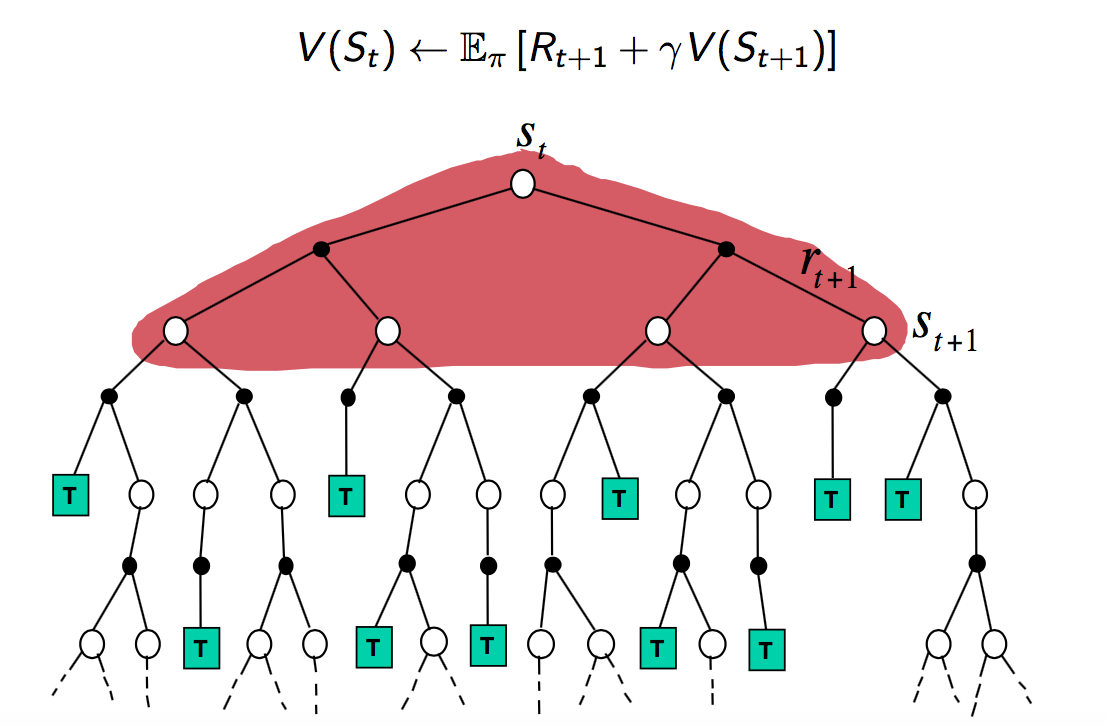
\includegraphics[width=0.60\textwidth]{figures/dynamic_programming_backup.png}
	\label{fig:DP}
\end{figure}


\end{frame}

\section{Example: Invest or Save?}
{
\setbeamercolor{background canvas}{bg=BrewerBlue}
\begin{frame}
\centering
\Huge
\textcolor{white}{Example: Invest or Save?}
\thispagestyle{empty}
\end{frame}
}

\begin{frame}{A Markov Decision Process}

\scalebox{0.7}{
\tikz{

\tikzstyle{mystyle}=[draw=BrewerBlue, circle, inner sep=0pt, minimum size=1.7cm, line width=1pt, fill=BrewerBlue!20!white, align=center, font=\footnotesize,]

\tikzset{>={Latex[length=1.75mm,width=1.25mm]}}

% Circles
\node[mystyle] (p1) {Poor \&\\Unknown\\$\textcolor{red1}{+0}$};
\node[mystyle, right=5cm of p1] (p2) {Poor \&\\Famous\\$\textcolor{red1}{+0}$};

\node[mystyle, below=3cm of p1] (r1) {Rich \&\\Unknown\\$\textcolor{red1}{+10}$};
\node[mystyle] (r2) at (r1-|p2) {Rich \&\\Famous\\$\textcolor{red1}{+10}$};

% Big Arrows
\begin{scope}[on behind layer]
\node[single arrow, draw=red1, fill=none, minimum width = 16pt, line width=1pt, single arrow head extend=3pt, minimum height=10mm, inner sep=1.5pt, anchor=west] (p1a) at ($(p1.east)+(-.1,0)$) {\scriptsize I};  

\node[single arrow, draw=red1, fill=none, minimum width = 16pt, line width=1pt, single arrow head extend=3pt, minimum height=10mm, inner sep=1.85pt, anchor=west, rotate=90] (p1s) at ($(p1.north)+(0,-.1)$) {\scriptsize\rotatebox{-90}{S}}; 

%---
\node[single arrow, draw=red1, fill=none, minimum width = 16pt, line width=1pt, single arrow head extend=3pt, minimum height=10mm, inner sep=1.5pt, anchor=west] (p2a) at ($(p2.east)+(-.1,0)$) {\scriptsize I};  

\node[single arrow, draw=red1, fill=none, minimum width = 16pt, line width=1pt, single arrow head extend=3pt, minimum height=10mm, inner sep=1.85pt, anchor=west, rotate=-90] (p2s) at ($(p2.south)+(0,.1)$) {\scriptsize\rotatebox{90}{S}}; 

%---
\node[single arrow, draw=red1, fill=none, minimum width = 16pt, line width=1pt, single arrow head extend=3pt, minimum height=10mm, inner sep=1.5pt, anchor=west, rotate=45] (r1a) at ($(r1.45)+(-.1,-.1)$) {\scriptsize I}; 

\node[single arrow, draw=red1, fill=none, minimum width = 16pt, line width=1pt, single arrow head extend=3pt, minimum height=10mm, inner sep=1.5pt, anchor=west, rotate=90+45] (r1s) at ($(r1.90+45)+(.1,-.1)$) {\scriptsize S}; 

%---
\node[single arrow, draw=red1, fill=none, minimum width = 16pt, line width=1pt, single arrow head extend=3pt, minimum height=10mm, inner sep=1.5pt, anchor=west, rotate=45] (r2a) at ($(r2.45)+(-.1,-.1)$) {\scriptsize I}; 

\node[single arrow, draw=red1, fill=none, minimum width = 16pt, line width=1pt, single arrow head extend=3pt, minimum height=10mm, inner sep=1.5pt, anchor=west, rotate=180] (r2s) at ($(r2.west)+(.1,0)$) {\scriptsize \rotatebox{180}{S}}; 
\end{scope}

%------Arrows 
% Loops
\draw[->] (p1s.20) to[out=150, in=150, looseness=1.75] node[above left=-1mm] {\small $1$} (p1.160);

\draw[->] (p1a.20) to[out=70, in=60, looseness=1.75] node[above] {$\sfrac{1}{2}$} (p1.45);

\draw[->] (p2a.20) to[out=70, in=60, looseness=1.75] node[above] {\small $1$} (p2.90);

\draw[->] (r1s.20) to[out=200, in=-160, looseness=1.75] node[below left=-1mm] {$\sfrac{1}{2}$} (r1.south west);

\draw[->] (r2s.20) to[out=240, in=-120, looseness=1.75] node[below left=-1mm] {$\sfrac{1}{2}$} (r2.-110);

% Direct paths
\draw[->] (r1s.-20) to[out=120, in=-140, looseness=1] node[left=0mm] {$\sfrac{1}{2}$} (p1.-130);

\draw[->] (r1a.20) to[out=120, in=-90, looseness=1] node[left=0mm] {$\sfrac{1}{2}$} (p1.-90);

\draw[->] (r1a.east) to[out=40, in=180, looseness=1] node[above left=-1mm, pos=.2] {$\sfrac{1}{2}$} (p2.west);

\draw[->] (r2s.east) to[out=180, in=-30, looseness=1] node[above left=-1mm, pos=.2] {$\sfrac{1}{2}$} (r1.south east);

\draw[->] (r2a.east) to[out=60, in=-30, looseness=1] node[above right=0mm, pos=.2] {\small $1$} (p2.south east);

\draw[->] (p2s.-10) to[out=230, in=90+45, looseness=1] node[left=0mm, pos=.5] {$\sfrac{1}{2}$} (r2.north west);

\draw[->] (p2s.-30) to[out=180, in=-45, looseness=1] node[above=0mm, pos=.2] {$\sfrac{1}{2}$} (p1.south east);

\draw[->] (p1a.10) to[out=30, in=90+45, looseness=1] node[above=0mm, pos=.5] {$\sfrac{1}{2}$} (p2.north west);

}
}

You own a company

In every state you must choose between \textbf{I}nvesting or \textbf{S}aving.\\
$\gamma=0.9$
\vspace*{18pt}
\end{frame}


\begin{frame}{Transition Model for Invest}
\scalebox{0.7}{
\centering
\tikz{

\tikzstyle{mystyle}=[draw=BrewerBlue, circle, inner sep=0pt, minimum size=1.7cm, line width=1pt, fill=BrewerBlue!20!white, align=center, font=\footnotesize,]

\tikzset{>={Latex[length=1.75mm,width=1.25mm]}}

% Circles
\node[mystyle] (p1) {Poor \&\\Unknown\\$\textcolor{red1}{+0}$};
\node[mystyle, right=5cm of p1] (p2) {Poor \&\\Famous\\$\textcolor{red1}{+0}$};

\node[mystyle, below=3cm of p1] (r1) {Rich \&\\Unknown\\$\textcolor{red1}{+10}$};
\node[mystyle] (r2) at (r1-|p2) {Rich \&\\Famous\\$\textcolor{red1}{+10}$};

% Big Arrows
\begin{scope}[on behind layer]
\node[single arrow, draw=red1, fill=none, minimum width = 16pt, line width=1pt, single arrow head extend=3pt, minimum height=10mm, inner sep=1.5pt, anchor=west] (p1a) at ($(p1.east)+(-.1,0)$) {\scriptsize I};  

\node[single arrow, draw=red1, fill=none, minimum width = 16pt, line width=1pt, single arrow head extend=3pt, minimum height=10mm, inner sep=1.85pt, anchor=west, rotate=90] (p1s) at ($(p1.north)+(0,-.1)$) {\scriptsize\rotatebox{-90}{S}}; 

%---
\node[single arrow, draw=red1, fill=none, minimum width = 16pt, line width=1pt, single arrow head extend=3pt, minimum height=10mm, inner sep=1.5pt, anchor=west] (p2a) at ($(p2.east)+(-.1,0)$) {\scriptsize I};  

\node[single arrow, draw=red1, fill=none, minimum width = 16pt, line width=1pt, single arrow head extend=3pt, minimum height=10mm, inner sep=1.85pt, anchor=west, rotate=-90] (p2s) at ($(p2.south)+(0,.1)$) {\scriptsize\rotatebox{90}{S}}; 

%---
\node[single arrow, draw=red1, fill=none, minimum width = 16pt, line width=1pt, single arrow head extend=3pt, minimum height=10mm, inner sep=1.5pt, anchor=west, rotate=45] (r1a) at ($(r1.45)+(-.1,-.1)$) {\scriptsize I}; 

\node[single arrow, draw=red1, fill=none, minimum width = 16pt, line width=1pt, single arrow head extend=3pt, minimum height=10mm, inner sep=1.5pt, anchor=west, rotate=90+45] (r1s) at ($(r1.90+45)+(.1,-.1)$) {\scriptsize S}; 

%---
\node[single arrow, draw=red1, fill=none, minimum width = 16pt, line width=1pt, single arrow head extend=3pt, minimum height=10mm, inner sep=1.5pt, anchor=west, rotate=45] (r2a) at ($(r2.45)+(-.1,-.1)$) {\scriptsize I}; 

\node[single arrow, draw=red1, fill=none, minimum width = 16pt, line width=1pt, single arrow head extend=3pt, minimum height=10mm, inner sep=1.5pt, anchor=west, rotate=180] (r2s) at ($(r2.west)+(.1,0)$) {\scriptsize \rotatebox{180}{S}}; 
\end{scope}

%------Arrows 
% Loops
\draw[->] (p1s.20) to[out=150, in=150, looseness=1.75] node[above left=-1mm] {\small $1$} (p1.160);

\draw[->] (p1a.20) to[out=70, in=60, looseness=1.75] node[above] {$\sfrac{1}{2}$} (p1.45);

\draw[->] (p2a.20) to[out=70, in=60, looseness=1.75] node[above] {\small $1$} (p2.90);

\draw[->] (r1s.20) to[out=200, in=-160, looseness=1.75] node[below left=-1mm] {$\sfrac{1}{2}$} (r1.south west);

\draw[->] (r2s.20) to[out=240, in=-120, looseness=1.75] node[below left=-1mm] {$\sfrac{1}{2}$} (r2.-110);

% Direct paths
\draw[->] (r1s.-20) to[out=120, in=-140, looseness=1] node[left=0mm] {$\sfrac{1}{2}$} (p1.-130);

\draw[->] (r1a.20) to[out=120, in=-90, looseness=1] node[left=0mm] {$\sfrac{1}{2}$} (p1.-90);

\draw[->] (r1a.east) to[out=40, in=180, looseness=1] node[above left=-1mm, pos=.2] {$\sfrac{1}{2}$} (p2.west);

\draw[->] (r2s.east) to[out=180, in=-30, looseness=1] node[above left=-1mm, pos=.2] {$\sfrac{1}{2}$} (r1.south east);

\draw[->] (r2a.east) to[out=60, in=-30, looseness=1] node[above right=0mm, pos=.2] {\small $1$} (p2.south east);

\draw[->] (p2s.-10) to[out=230, in=90+45, looseness=1] node[left=0mm, pos=.5] {$\sfrac{1}{2}$} (r2.north west);

\draw[->] (p2s.-30) to[out=180, in=-45, looseness=1] node[above=0mm, pos=.2] {$\sfrac{1}{2}$} (p1.south east);

\draw[->] (p1a.10) to[out=30, in=90+45, looseness=1] node[above=0mm, pos=.5] {$\sfrac{1}{2}$} (p2.north west);

}
}

\begin{figure}
		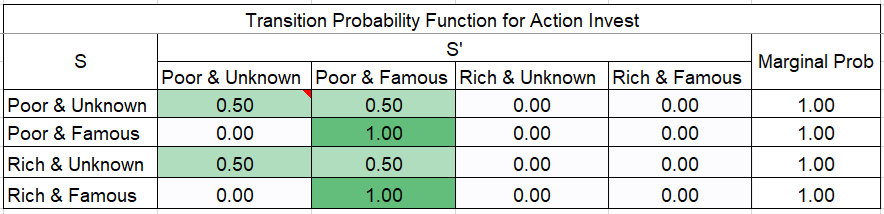
\includegraphics[width=0.70\textwidth]{figures/transitions_invest.png}
	\label{fig:transitions_invest}
\end{figure}

\end{frame}

\begin{frame}{Reward Model for Invest}
\scalebox{0.7}{
\centering
\tikz{

\tikzstyle{mystyle}=[draw=BrewerBlue, circle, inner sep=0pt, minimum size=1.7cm, line width=1pt, fill=BrewerBlue!20!white, align=center, font=\footnotesize,]

\tikzset{>={Latex[length=1.75mm,width=1.25mm]}}

% Circles
\node[mystyle] (p1) {Poor \&\\Unknown\\$\textcolor{red1}{+0}$};
\node[mystyle, right=5cm of p1] (p2) {Poor \&\\Famous\\$\textcolor{red1}{+0}$};

\node[mystyle, below=3cm of p1] (r1) {Rich \&\\Unknown\\$\textcolor{red1}{+10}$};
\node[mystyle] (r2) at (r1-|p2) {Rich \&\\Famous\\$\textcolor{red1}{+10}$};

% Big Arrows
\begin{scope}[on behind layer]
\node[single arrow, draw=red1, fill=none, minimum width = 16pt, line width=1pt, single arrow head extend=3pt, minimum height=10mm, inner sep=1.5pt, anchor=west] (p1a) at ($(p1.east)+(-.1,0)$) {\scriptsize I};  

\node[single arrow, draw=red1, fill=none, minimum width = 16pt, line width=1pt, single arrow head extend=3pt, minimum height=10mm, inner sep=1.85pt, anchor=west, rotate=90] (p1s) at ($(p1.north)+(0,-.1)$) {\scriptsize\rotatebox{-90}{S}}; 

%---
\node[single arrow, draw=red1, fill=none, minimum width = 16pt, line width=1pt, single arrow head extend=3pt, minimum height=10mm, inner sep=1.5pt, anchor=west] (p2a) at ($(p2.east)+(-.1,0)$) {\scriptsize I};  

\node[single arrow, draw=red1, fill=none, minimum width = 16pt, line width=1pt, single arrow head extend=3pt, minimum height=10mm, inner sep=1.85pt, anchor=west, rotate=-90] (p2s) at ($(p2.south)+(0,.1)$) {\scriptsize\rotatebox{90}{S}}; 

%---
\node[single arrow, draw=red1, fill=none, minimum width = 16pt, line width=1pt, single arrow head extend=3pt, minimum height=10mm, inner sep=1.5pt, anchor=west, rotate=45] (r1a) at ($(r1.45)+(-.1,-.1)$) {\scriptsize I}; 

\node[single arrow, draw=red1, fill=none, minimum width = 16pt, line width=1pt, single arrow head extend=3pt, minimum height=10mm, inner sep=1.5pt, anchor=west, rotate=90+45] (r1s) at ($(r1.90+45)+(.1,-.1)$) {\scriptsize S}; 

%---
\node[single arrow, draw=red1, fill=none, minimum width = 16pt, line width=1pt, single arrow head extend=3pt, minimum height=10mm, inner sep=1.5pt, anchor=west, rotate=45] (r2a) at ($(r2.45)+(-.1,-.1)$) {\scriptsize I}; 

\node[single arrow, draw=red1, fill=none, minimum width = 16pt, line width=1pt, single arrow head extend=3pt, minimum height=10mm, inner sep=1.5pt, anchor=west, rotate=180] (r2s) at ($(r2.west)+(.1,0)$) {\scriptsize \rotatebox{180}{S}}; 
\end{scope}

%------Arrows 
% Loops
\draw[->] (p1s.20) to[out=150, in=150, looseness=1.75] node[above left=-1mm] {\small $1$} (p1.160);

\draw[->] (p1a.20) to[out=70, in=60, looseness=1.75] node[above] {$\sfrac{1}{2}$} (p1.45);

\draw[->] (p2a.20) to[out=70, in=60, looseness=1.75] node[above] {\small $1$} (p2.90);

\draw[->] (r1s.20) to[out=200, in=-160, looseness=1.75] node[below left=-1mm] {$\sfrac{1}{2}$} (r1.south west);

\draw[->] (r2s.20) to[out=240, in=-120, looseness=1.75] node[below left=-1mm] {$\sfrac{1}{2}$} (r2.-110);

% Direct paths
\draw[->] (r1s.-20) to[out=120, in=-140, looseness=1] node[left=0mm] {$\sfrac{1}{2}$} (p1.-130);

\draw[->] (r1a.20) to[out=120, in=-90, looseness=1] node[left=0mm] {$\sfrac{1}{2}$} (p1.-90);

\draw[->] (r1a.east) to[out=40, in=180, looseness=1] node[above left=-1mm, pos=.2] {$\sfrac{1}{2}$} (p2.west);

\draw[->] (r2s.east) to[out=180, in=-30, looseness=1] node[above left=-1mm, pos=.2] {$\sfrac{1}{2}$} (r1.south east);

\draw[->] (r2a.east) to[out=60, in=-30, looseness=1] node[above right=0mm, pos=.2] {\small $1$} (p2.south east);

\draw[->] (p2s.-10) to[out=230, in=90+45, looseness=1] node[left=0mm, pos=.5] {$\sfrac{1}{2}$} (r2.north west);

\draw[->] (p2s.-30) to[out=180, in=-45, looseness=1] node[above=0mm, pos=.2] {$\sfrac{1}{2}$} (p1.south east);

\draw[->] (p1a.10) to[out=30, in=90+45, looseness=1] node[above=0mm, pos=.5] {$\sfrac{1}{2}$} (p2.north west);

}
}

\begin{figure}
		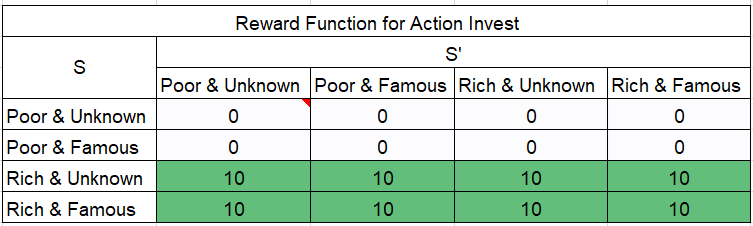
\includegraphics[width=0.60\textwidth]{figures/rewards_invest.png}
	\label{fig:rewards_invest}
\end{figure}

\end{frame}

\begin{frame}{Transition Model for Save}
\scalebox{0.7}{
\centering
\tikz{

\tikzstyle{mystyle}=[draw=BrewerBlue, circle, inner sep=0pt, minimum size=1.7cm, line width=1pt, fill=BrewerBlue!20!white, align=center, font=\footnotesize,]

\tikzset{>={Latex[length=1.75mm,width=1.25mm]}}

% Circles
\node[mystyle] (p1) {Poor \&\\Unknown\\$\textcolor{red1}{+0}$};
\node[mystyle, right=5cm of p1] (p2) {Poor \&\\Famous\\$\textcolor{red1}{+0}$};

\node[mystyle, below=3cm of p1] (r1) {Rich \&\\Unknown\\$\textcolor{red1}{+10}$};
\node[mystyle] (r2) at (r1-|p2) {Rich \&\\Famous\\$\textcolor{red1}{+10}$};

% Big Arrows
\begin{scope}[on behind layer]
\node[single arrow, draw=red1, fill=none, minimum width = 16pt, line width=1pt, single arrow head extend=3pt, minimum height=10mm, inner sep=1.5pt, anchor=west] (p1a) at ($(p1.east)+(-.1,0)$) {\scriptsize I};  

\node[single arrow, draw=red1, fill=none, minimum width = 16pt, line width=1pt, single arrow head extend=3pt, minimum height=10mm, inner sep=1.85pt, anchor=west, rotate=90] (p1s) at ($(p1.north)+(0,-.1)$) {\scriptsize\rotatebox{-90}{S}}; 

%---
\node[single arrow, draw=red1, fill=none, minimum width = 16pt, line width=1pt, single arrow head extend=3pt, minimum height=10mm, inner sep=1.5pt, anchor=west] (p2a) at ($(p2.east)+(-.1,0)$) {\scriptsize I};  

\node[single arrow, draw=red1, fill=none, minimum width = 16pt, line width=1pt, single arrow head extend=3pt, minimum height=10mm, inner sep=1.85pt, anchor=west, rotate=-90] (p2s) at ($(p2.south)+(0,.1)$) {\scriptsize\rotatebox{90}{S}}; 

%---
\node[single arrow, draw=red1, fill=none, minimum width = 16pt, line width=1pt, single arrow head extend=3pt, minimum height=10mm, inner sep=1.5pt, anchor=west, rotate=45] (r1a) at ($(r1.45)+(-.1,-.1)$) {\scriptsize I}; 

\node[single arrow, draw=red1, fill=none, minimum width = 16pt, line width=1pt, single arrow head extend=3pt, minimum height=10mm, inner sep=1.5pt, anchor=west, rotate=90+45] (r1s) at ($(r1.90+45)+(.1,-.1)$) {\scriptsize S}; 

%---
\node[single arrow, draw=red1, fill=none, minimum width = 16pt, line width=1pt, single arrow head extend=3pt, minimum height=10mm, inner sep=1.5pt, anchor=west, rotate=45] (r2a) at ($(r2.45)+(-.1,-.1)$) {\scriptsize I}; 

\node[single arrow, draw=red1, fill=none, minimum width = 16pt, line width=1pt, single arrow head extend=3pt, minimum height=10mm, inner sep=1.5pt, anchor=west, rotate=180] (r2s) at ($(r2.west)+(.1,0)$) {\scriptsize \rotatebox{180}{S}}; 
\end{scope}

%------Arrows 
% Loops
\draw[->] (p1s.20) to[out=150, in=150, looseness=1.75] node[above left=-1mm] {\small $1$} (p1.160);

\draw[->] (p1a.20) to[out=70, in=60, looseness=1.75] node[above] {$\sfrac{1}{2}$} (p1.45);

\draw[->] (p2a.20) to[out=70, in=60, looseness=1.75] node[above] {\small $1$} (p2.90);

\draw[->] (r1s.20) to[out=200, in=-160, looseness=1.75] node[below left=-1mm] {$\sfrac{1}{2}$} (r1.south west);

\draw[->] (r2s.20) to[out=240, in=-120, looseness=1.75] node[below left=-1mm] {$\sfrac{1}{2}$} (r2.-110);

% Direct paths
\draw[->] (r1s.-20) to[out=120, in=-140, looseness=1] node[left=0mm] {$\sfrac{1}{2}$} (p1.-130);

\draw[->] (r1a.20) to[out=120, in=-90, looseness=1] node[left=0mm] {$\sfrac{1}{2}$} (p1.-90);

\draw[->] (r1a.east) to[out=40, in=180, looseness=1] node[above left=-1mm, pos=.2] {$\sfrac{1}{2}$} (p2.west);

\draw[->] (r2s.east) to[out=180, in=-30, looseness=1] node[above left=-1mm, pos=.2] {$\sfrac{1}{2}$} (r1.south east);

\draw[->] (r2a.east) to[out=60, in=-30, looseness=1] node[above right=0mm, pos=.2] {\small $1$} (p2.south east);

\draw[->] (p2s.-10) to[out=230, in=90+45, looseness=1] node[left=0mm, pos=.5] {$\sfrac{1}{2}$} (r2.north west);

\draw[->] (p2s.-30) to[out=180, in=-45, looseness=1] node[above=0mm, pos=.2] {$\sfrac{1}{2}$} (p1.south east);

\draw[->] (p1a.10) to[out=30, in=90+45, looseness=1] node[above=0mm, pos=.5] {$\sfrac{1}{2}$} (p2.north west);

}
}

\begin{figure}
		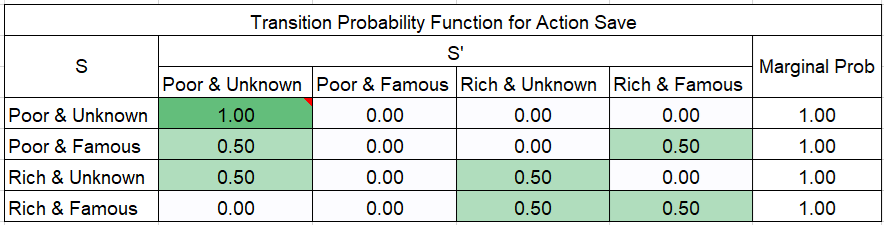
\includegraphics[width=0.70\textwidth]{figures/transitions_save.png}
	\label{fig:transitions_save}
\end{figure}

\end{frame}

\begin{frame}{Reward Model for Save}
\scalebox{0.7}{
\centering
\tikz{

\tikzstyle{mystyle}=[draw=BrewerBlue, circle, inner sep=0pt, minimum size=1.7cm, line width=1pt, fill=BrewerBlue!20!white, align=center, font=\footnotesize,]

\tikzset{>={Latex[length=1.75mm,width=1.25mm]}}

% Circles
\node[mystyle] (p1) {Poor \&\\Unknown\\$\textcolor{red1}{+0}$};
\node[mystyle, right=5cm of p1] (p2) {Poor \&\\Famous\\$\textcolor{red1}{+0}$};

\node[mystyle, below=3cm of p1] (r1) {Rich \&\\Unknown\\$\textcolor{red1}{+10}$};
\node[mystyle] (r2) at (r1-|p2) {Rich \&\\Famous\\$\textcolor{red1}{+10}$};

% Big Arrows
\begin{scope}[on behind layer]
\node[single arrow, draw=red1, fill=none, minimum width = 16pt, line width=1pt, single arrow head extend=3pt, minimum height=10mm, inner sep=1.5pt, anchor=west] (p1a) at ($(p1.east)+(-.1,0)$) {\scriptsize I};  

\node[single arrow, draw=red1, fill=none, minimum width = 16pt, line width=1pt, single arrow head extend=3pt, minimum height=10mm, inner sep=1.85pt, anchor=west, rotate=90] (p1s) at ($(p1.north)+(0,-.1)$) {\scriptsize\rotatebox{-90}{S}}; 

%---
\node[single arrow, draw=red1, fill=none, minimum width = 16pt, line width=1pt, single arrow head extend=3pt, minimum height=10mm, inner sep=1.5pt, anchor=west] (p2a) at ($(p2.east)+(-.1,0)$) {\scriptsize I};  

\node[single arrow, draw=red1, fill=none, minimum width = 16pt, line width=1pt, single arrow head extend=3pt, minimum height=10mm, inner sep=1.85pt, anchor=west, rotate=-90] (p2s) at ($(p2.south)+(0,.1)$) {\scriptsize\rotatebox{90}{S}}; 

%---
\node[single arrow, draw=red1, fill=none, minimum width = 16pt, line width=1pt, single arrow head extend=3pt, minimum height=10mm, inner sep=1.5pt, anchor=west, rotate=45] (r1a) at ($(r1.45)+(-.1,-.1)$) {\scriptsize I}; 

\node[single arrow, draw=red1, fill=none, minimum width = 16pt, line width=1pt, single arrow head extend=3pt, minimum height=10mm, inner sep=1.5pt, anchor=west, rotate=90+45] (r1s) at ($(r1.90+45)+(.1,-.1)$) {\scriptsize S}; 

%---
\node[single arrow, draw=red1, fill=none, minimum width = 16pt, line width=1pt, single arrow head extend=3pt, minimum height=10mm, inner sep=1.5pt, anchor=west, rotate=45] (r2a) at ($(r2.45)+(-.1,-.1)$) {\scriptsize I}; 

\node[single arrow, draw=red1, fill=none, minimum width = 16pt, line width=1pt, single arrow head extend=3pt, minimum height=10mm, inner sep=1.5pt, anchor=west, rotate=180] (r2s) at ($(r2.west)+(.1,0)$) {\scriptsize \rotatebox{180}{S}}; 
\end{scope}

%------Arrows 
% Loops
\draw[->] (p1s.20) to[out=150, in=150, looseness=1.75] node[above left=-1mm] {\small $1$} (p1.160);

\draw[->] (p1a.20) to[out=70, in=60, looseness=1.75] node[above] {$\sfrac{1}{2}$} (p1.45);

\draw[->] (p2a.20) to[out=70, in=60, looseness=1.75] node[above] {\small $1$} (p2.90);

\draw[->] (r1s.20) to[out=200, in=-160, looseness=1.75] node[below left=-1mm] {$\sfrac{1}{2}$} (r1.south west);

\draw[->] (r2s.20) to[out=240, in=-120, looseness=1.75] node[below left=-1mm] {$\sfrac{1}{2}$} (r2.-110);

% Direct paths
\draw[->] (r1s.-20) to[out=120, in=-140, looseness=1] node[left=0mm] {$\sfrac{1}{2}$} (p1.-130);

\draw[->] (r1a.20) to[out=120, in=-90, looseness=1] node[left=0mm] {$\sfrac{1}{2}$} (p1.-90);

\draw[->] (r1a.east) to[out=40, in=180, looseness=1] node[above left=-1mm, pos=.2] {$\sfrac{1}{2}$} (p2.west);

\draw[->] (r2s.east) to[out=180, in=-30, looseness=1] node[above left=-1mm, pos=.2] {$\sfrac{1}{2}$} (r1.south east);

\draw[->] (r2a.east) to[out=60, in=-30, looseness=1] node[above right=0mm, pos=.2] {\small $1$} (p2.south east);

\draw[->] (p2s.-10) to[out=230, in=90+45, looseness=1] node[left=0mm, pos=.5] {$\sfrac{1}{2}$} (r2.north west);

\draw[->] (p2s.-30) to[out=180, in=-45, looseness=1] node[above=0mm, pos=.2] {$\sfrac{1}{2}$} (p1.south east);

\draw[->] (p1a.10) to[out=30, in=90+45, looseness=1] node[above=0mm, pos=.5] {$\sfrac{1}{2}$} (p2.north west);

}
}

\begin{figure}
		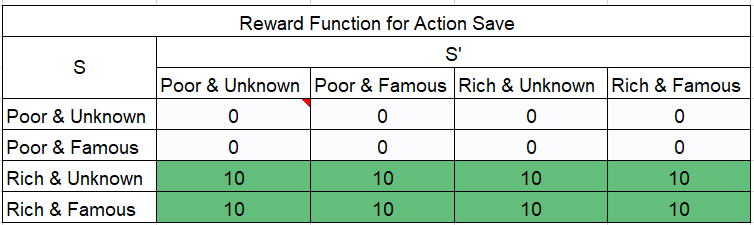
\includegraphics[width=0.60\textwidth]{figures/rewards_save.png}
	\label{fig:rewards_save}
\end{figure}

\end{frame}



\begin{frame}{Values and Policies for Each State}
\centering
\scalebox{0.5}{
\tikz{

\tikzstyle{mystyle}=[draw=BrewerBlue, circle, inner sep=0pt, minimum size=1.7cm, line width=1pt, fill=BrewerBlue!20!white, align=center, font=\footnotesize,]

\tikzset{>={Latex[length=1.75mm,width=1.25mm]}}

% Circles
\node[mystyle] (p1) {Poor \&\\Unknown\\$\textcolor{red1}{+0}$};
\node[mystyle, right=5cm of p1] (p2) {Poor \&\\Famous\\$\textcolor{red1}{+0}$};

\node[mystyle, below=3cm of p1] (r1) {Rich \&\\Unknown\\$\textcolor{red1}{+10}$};
\node[mystyle] (r2) at (r1-|p2) {Rich \&\\Famous\\$\textcolor{red1}{+10}$};

% Big Arrows
\begin{scope}[on behind layer]
\node[single arrow, draw=red1, fill=none, minimum width = 16pt, line width=1pt, single arrow head extend=3pt, minimum height=10mm, inner sep=1.5pt, anchor=west] (p1a) at ($(p1.east)+(-.1,0)$) {\scriptsize I};  

\node[single arrow, draw=red1, fill=none, minimum width = 16pt, line width=1pt, single arrow head extend=3pt, minimum height=10mm, inner sep=1.85pt, anchor=west, rotate=90] (p1s) at ($(p1.north)+(0,-.1)$) {\scriptsize\rotatebox{-90}{S}}; 

%---
\node[single arrow, draw=red1, fill=none, minimum width = 16pt, line width=1pt, single arrow head extend=3pt, minimum height=10mm, inner sep=1.5pt, anchor=west] (p2a) at ($(p2.east)+(-.1,0)$) {\scriptsize I};  

\node[single arrow, draw=red1, fill=none, minimum width = 16pt, line width=1pt, single arrow head extend=3pt, minimum height=10mm, inner sep=1.85pt, anchor=west, rotate=-90] (p2s) at ($(p2.south)+(0,.1)$) {\scriptsize\rotatebox{90}{S}}; 

%---
\node[single arrow, draw=red1, fill=none, minimum width = 16pt, line width=1pt, single arrow head extend=3pt, minimum height=10mm, inner sep=1.5pt, anchor=west, rotate=45] (r1a) at ($(r1.45)+(-.1,-.1)$) {\scriptsize I}; 

\node[single arrow, draw=red1, fill=none, minimum width = 16pt, line width=1pt, single arrow head extend=3pt, minimum height=10mm, inner sep=1.5pt, anchor=west, rotate=90+45] (r1s) at ($(r1.90+45)+(.1,-.1)$) {\scriptsize S}; 

%---
\node[single arrow, draw=red1, fill=none, minimum width = 16pt, line width=1pt, single arrow head extend=3pt, minimum height=10mm, inner sep=1.5pt, anchor=west, rotate=45] (r2a) at ($(r2.45)+(-.1,-.1)$) {\scriptsize I}; 

\node[single arrow, draw=red1, fill=none, minimum width = 16pt, line width=1pt, single arrow head extend=3pt, minimum height=10mm, inner sep=1.5pt, anchor=west, rotate=180] (r2s) at ($(r2.west)+(.1,0)$) {\scriptsize \rotatebox{180}{S}}; 
\end{scope}

%------Arrows 
% Loops
\draw[->] (p1s.20) to[out=150, in=150, looseness=1.75] node[above left=-1mm] {\small $1$} (p1.160);

\draw[->] (p1a.20) to[out=70, in=60, looseness=1.75] node[above] {$\sfrac{1}{2}$} (p1.45);

\draw[->] (p2a.20) to[out=70, in=60, looseness=1.75] node[above] {\small $1$} (p2.90);

\draw[->] (r1s.20) to[out=200, in=-160, looseness=1.75] node[below left=-1mm] {$\sfrac{1}{2}$} (r1.south west);

\draw[->] (r2s.20) to[out=240, in=-120, looseness=1.75] node[below left=-1mm] {$\sfrac{1}{2}$} (r2.-110);

% Direct paths
\draw[->] (r1s.-20) to[out=120, in=-140, looseness=1] node[left=0mm] {$\sfrac{1}{2}$} (p1.-130);

\draw[->] (r1a.20) to[out=120, in=-90, looseness=1] node[left=0mm] {$\sfrac{1}{2}$} (p1.-90);

\draw[->] (r1a.east) to[out=40, in=180, looseness=1] node[above left=-1mm, pos=.2] {$\sfrac{1}{2}$} (p2.west);

\draw[->] (r2s.east) to[out=180, in=-30, looseness=1] node[above left=-1mm, pos=.2] {$\sfrac{1}{2}$} (r1.south east);

\draw[->] (r2a.east) to[out=60, in=-30, looseness=1] node[above right=0mm, pos=.2] {\small $1$} (p2.south east);

\draw[->] (p2s.-10) to[out=230, in=90+45, looseness=1] node[left=0mm, pos=.5] {$\sfrac{1}{2}$} (r2.north west);

\draw[->] (p2s.-30) to[out=180, in=-45, looseness=1] node[above=0mm, pos=.2] {$\sfrac{1}{2}$} (p1.south east);

\draw[->] (p1a.10) to[out=30, in=90+45, looseness=1] node[above=0mm, pos=.5] {$\sfrac{1}{2}$} (p2.north west);

}
}
\footnotesize
$$
\begin{gathered}
V_{h}(R F)=\max _{\text {action }}\{R(R F, I), R(R F, S)\}=\max _{a}\{10,10\}=10 \\
\pi_{h}(R F)=\operatorname{argmax}\{R(R F, I), R(R F, S)\}=\{I, S\}
\end{gathered}
$$

$$
\begin{gathered}
V_{h-1}(R F)=\max _{\text {action }} R(R F, \text { action })+\gamma \sum_{\text {state }_{h}} \mathbb{P}\left(s_{h} \mid R F, a_{h-1}\right) V\left(s_{h}\right)= \\
=\max _{\text {action }}\{10+0.9(1 * 0), 10+0.9(0.5 * 10+0.5 * 10)\}=\max _{a}\{10,19\}=19 \\
\pi_{h-1}(R F)=\{S\}
\end{gathered}
$$
    
\end{frame}



\begin{frame}{Values and Policies for Each State}

\footnotesize
$$
\begin{gathered}
V_{h}(R F)=\max _{\text {action }}\{R(R F, I), R(R F, S)\}=\max _{a}\{10,10\}=10 \\
\pi_{h}(R F)=\operatorname{argmax}\{R(R F, I), R(R F, S)\}=\{I, S\}
\end{gathered}
$$

$$
\begin{gathered}
V_{h-1}(R F)=\max _{\text {action }} R(R F, \text { action })+\gamma \sum_{\text {state }_{h}} \mathbb{P}\left(s_{h} \mid R F, a_{h-1}\right) V\left(s_{h}\right)= \\
=\max _{\text {action }}\{10+0.9(1 * 0), 10+0.9(0.5 * 10+0.5 * 10)\}=\max _{a}\{10,19\}=19 \\
\pi_{h-1}(R F)=\{S\}
\end{gathered}
$$

\begin{figure}
	\centering
		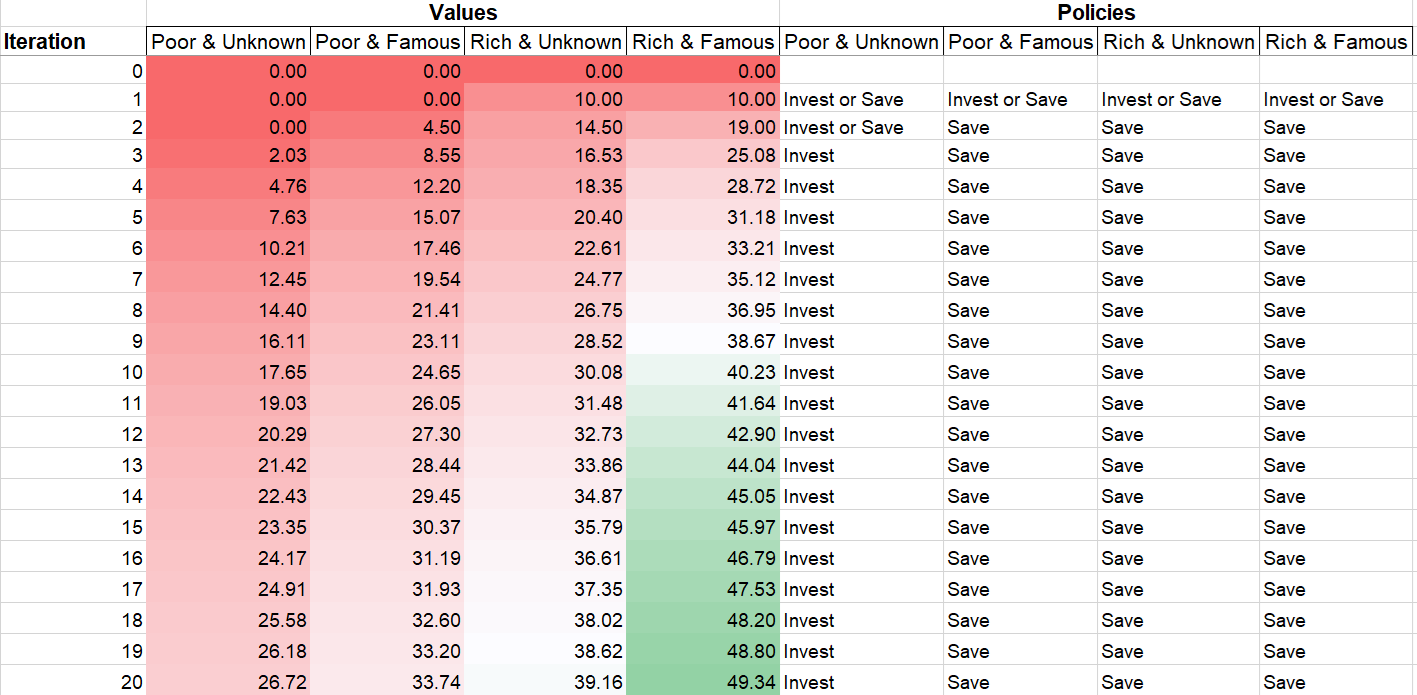
\includegraphics[width=0.80\textwidth]{figures/values_policies_convergence.png}
	\label{fig:values_policies_convergence}
\end{figure}

    
\end{frame}



\begin{frame}{Value Iteration Converges}

\footnotesize
$$
\begin{gathered}
V_{h}(R F)=\max _{\text {action }}\{R(R F, I), R(R F, S)\}=\max _{a}\{10,10\}=10 \\
\pi_{h}(R F)=\operatorname{argmax}\{R(R F, I), R(R F, S)\}=\{I, S\}
\end{gathered}
$$

$$
\begin{gathered}
V_{h-1}(R F)=\max _{\text {action }} R(R F, \text { action })+\gamma \sum_{\text {state }_{h}} \mathbb{P}\left(s_{h} \mid R F, a_{h-1}\right) V\left(s_{h}\right)= \\
=\max _{\text {action }}\{10+0.9(1 * 0), 10+0.9(0.5 * 10+0.5 * 10)\}=\max _{a}\{10,19\}=19 \\
\pi_{h-1}(R F)=\{S\}
\end{gathered}
$$

\begin{figure}
	\centering
		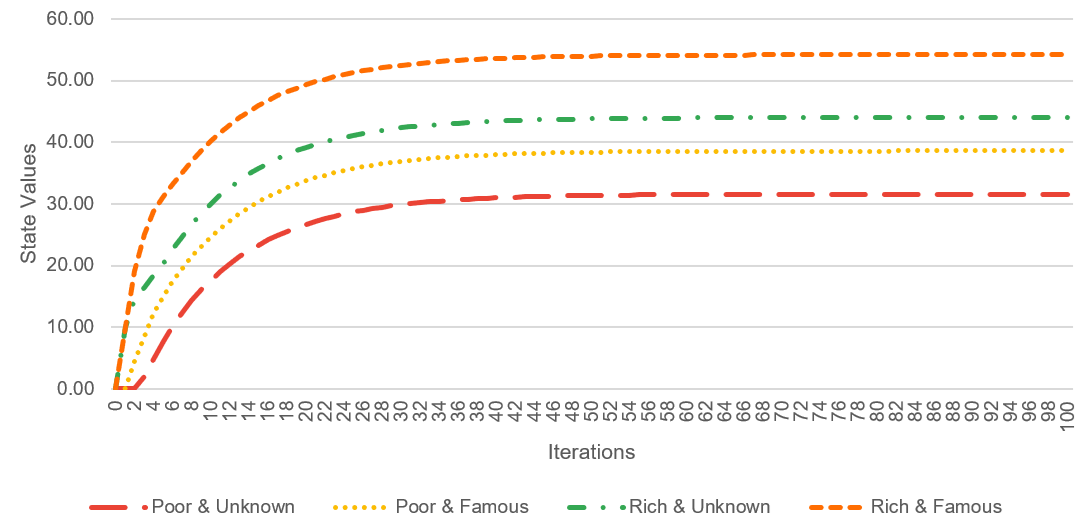
\includegraphics[width=0.80\textwidth]{figures/values_convergence.png}
	\label{fig:values_convergence}
\end{figure}

    
\end{frame}

\section{Endgame Effects}
{
\setbeamercolor{background canvas}{bg=BrewerBlue}
\begin{frame}
\centering
\Huge
\textcolor{white}{Endgame Effects}
\thispagestyle{empty}
\end{frame}
}

\begin{frame}{Finite Horizon}

\begin{itemize}
\item When $h$ is finite,
\item \textcolor{red1}{Non-stationary} optimal policy
\item Best action different at each time step
\item Intuition: best action varies with the amount of time  left
 
\end{itemize}
    
\end{frame}

\begin{frame}{Infinite Horizon}

\begin{itemize}
\item When $h$ is infinite,
\item \textcolor{red1}{Stationary} optimal policy
\item Same best action at each time step
\item Intuition: same (infinite) amount of time left at each  time step, hence same best action
\item \textcolor{red1}{Problem}: value iteration does an infinite number of  iterations...
\end{itemize}
    
\end{frame}
\begin{frame}{Infinite Horizon}

    \begin{itemize}
\item \textcolor{red1}{Problem}: value iteration does an infinite number of  iterations...
\item Assuming a discount factor $\gamma$, after $n$ time steps,  rewards are scaled down by $\gamma^n$
\item For large enough $n$, rewards become insignificant  since $\gamma^n\rightarrow0$
\item Solution:
 \begin{itemize}
     \item pick large enough $n$
\item run value iteration for $n$ steps
\item Execute policy found at the $n^{th}$ iteration
 
 \end{itemize}
    \end{itemize}
    
\end{frame}


\begin{frame}[t,allowframebreaks
]%\nocite{*}
\frametitle{References}
\small
\bibliography{bib}
\end{frame}
\section{Takeaways}
{
\setbeamercolor{background canvas}{bg=BrewerBlue}
\begin{frame}
\centering
\Huge
\textcolor{white}{Takeaways}
\thispagestyle{empty}
\end{frame}
}

\begin{frame}{How to Get The Best Now And in The Future?}
\begin{itemize}
		\item Bellman equation relates immediate rewards to future values
    \item Value iteration solves for optimal policies by dynamic programming
    \item Finite horizon problems lead to non-stationary policies
    \item Infinite horizon problems yield stationary policies, stabilized with discounting
		\end{itemize}
\end{frame}


\end{document}
